\documentclass[border={0.1cm 0.1cm 0.1cm 0.1cm}]{standalone}  %E,S,W,N

\usepackage{amssymb}
\usepackage{amsmath}
\usepackage{tikz}

%the arrangement of hinged ribs & sternum of birds permits large volume changes of the thorax in which lungs & air-sacs are located (Schmidt-Nielsen, How Animals Work, 1972)

\begin{document}
	
	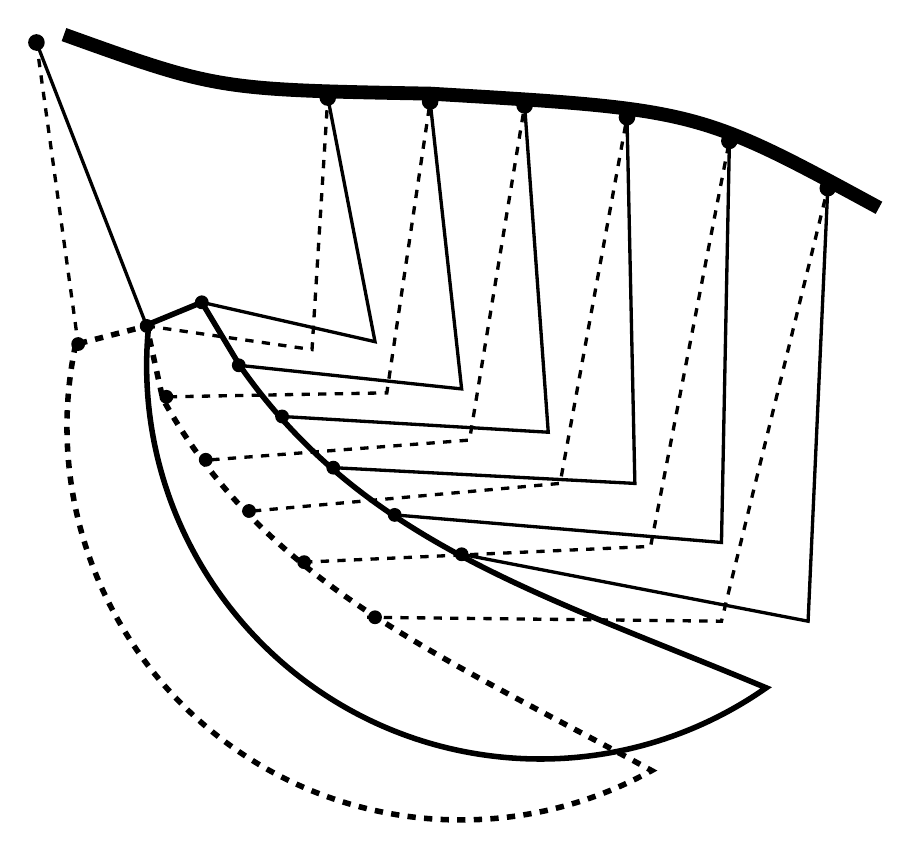
\begin{tikzpicture}[very thick]
	%TOP LINES
	\fill (-1.4,3.6) circle (3pt);
	\fill (-0.87,-0.23) circle (2.5pt);
	\draw[dashed] (-1.4,3.6)--(-0.87,-0.23);
	\draw (-1.4,3.6)--(0,0);
	\draw[line width=5] (-1.05,3.7) .. controls (0.9,3) .. (3.6,2.95) .. controls (7,2.75) .. (9.3,1.5);
	
	%CURVY SHAPE
	\draw[line width=2] ({5+5*cos(174)},{-0.5+5*sin(174)}) arc (174:305:5cm) .. controls (5,-3.4) and (2.75,-2.75) .. (0.28+0.9,-0.9+0.4)--(0.7,0.3)--cycle;
	%
	\draw[dashed,line width=2,rotate=-6] ({-0.9+5+5*cos(174)},{-0.35+-0.5+5*sin(174)}) arc (174:305:5cm) .. controls (-0.9+5,-3.4-0.35) and (-0.9+2.75,-2.75-0.35) .. (0.3,-0.9)--(0,0)--cycle;
	
	%LEFTMOST DOTS (DASHED LINE, LEFT)
	\fill (0,0) circle (2.5pt);
	\fill (0.25,-0.9) circle (2.5pt);
	\fill (0.75,-1.7) circle (2.5pt);
	\fill (1.3,-2.35) circle (2.5pt);
	\fill (2,-3) circle (2.5pt);
	\fill (2.9,-3.7) circle (2.5pt);
	
	%LEFTWARD DOTS (SOLID LINE, LEFT)
	\fill (0.7,0.3) circle (2.5pt);
	\fill (0.27+0.9,-0.9+0.4) circle (2.5pt);
	\fill (0.72+1,-1.7+0.55) circle (2.5pt);
	\fill (1.27+1.1,-2.35+0.55) circle (2.5pt);
	\fill (1.9+1.25,-3+0.6) circle (2.5pt);
	\fill (2.75+1.25,-3.7+0.8) circle (2.5pt);
	
	%SOLID HINGE
	\draw (0+0.7,0+0.3)--(2.9,-0.2)--(2.3,2.9);
	\draw (0.27+0.9,-0.9+0.4)--(4,-0.8)--(3.6,2.85);
	\draw (0.72+1,-1.7+0.55)--(5.1,-1.35)--(4.8,2.8);
	\draw (1.27+1.1,-2.35+0.55)--(6.2,-2)--(6.1,2.65);
	\draw (1.9+1.25,-3+0.6)--(7.3,-2.75)--(7.4,2.3);
	\draw (2.75+1.25,-3.7+0.8)--(8.4,-3.75)--(8.65,1.75);
	
	%DASHED HINGE
	\draw[dashed] (0,0)--(2.1,-0.3)--(2.3,2.9);
	\draw[dashed] (0.28,-0.9)--(3.05,-0.85)--(3.6,2.85);
	\draw[dashed] (0.82,-1.7)--(4.1,-1.45)--(4.8,2.8);
	\draw[dashed] (1.35,-2.35)--(5.25,-2)--(6.1,2.65);
	\draw[dashed] (2,-3)--(6.4,-2.8)--(7.4,2.35);
	\draw[dashed] (2.8,-3.7)--(7.3,-3.75)--(8.65,1.75);
	
	%RIGHTMOST DOTS
	\fill (2.3,2.9) circle (3pt);
	\fill (3.6,2.85) circle (3pt);
	\fill (4.8,2.8) circle (3pt);
	\fill (6.1,2.65) circle (3pt);
	\fill (7.4,2.35) circle (3pt);
	\fill (8.65,1.75) circle (3pt);
	\end{tikzpicture}
	
\end{document}